25. $\cfrac{(x^2-9)(y+x-1)}{x-3}=0\Leftrightarrow\cfrac{(x-3)(x+3)(y+x-1)}{x-3}=0\Leftrightarrow
\begin{cases}\left[\begin{array}{l}x=-3,\\ y=1-x.\end{array}\right.\\ x\neq3\end{cases}$
$$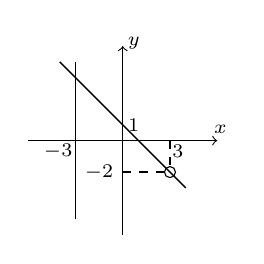
\begin{tikzpicture}[scale=0.2]
\tikzset {line01/.style={line width =0.5pt}}
\tikzset{line02/.style={line width =1pt}}
\tikzset{line03/.style={dashed,line width =0.5pt}}
%\filldraw [black] (0,0) circle (1pt);
\draw [->] (-6,0) -- (6,0);
\draw [->] (0,-6) -- (0,6);
\draw[line01] (-3,-5) -- (-3,5);
\draw[line01] (-4,5) -- (4,-3);
\draw (6.2,0.7) node {\scriptsize $x$};
\draw (-4.1,-0.7) node {\scriptsize $-3$};
\draw (3.5,-0.7) node {\scriptsize $3$};
\draw (0.7,1) node {\scriptsize $1$};
\draw (-1.5,-2) node {\scriptsize $-2$};
\draw[line03] (3,0) -- (3,-2);
\draw[line03] (0,-2) -- (3,-2);
\draw (0.7,6.2) node {\scriptsize $y$};
\draw (3,-2) circle (10pt);
\end{tikzpicture}$$
